\documentclass[a4paper]{article}
\paperheight=23cm
\paperwidth=18cm
\advance\textheight 10cm
\advance\topmargin -4.5cm
\advance\oddsidemargin -4cm
\usepackage{tikz}
\usetikzlibrary{decorations,decorations.pathmorphing,decorations.pathreplacing,shapes,snakes,arrows}
\usetikzlibrary{decorations.text}
\usepgflibrary{decorations.text}
\usetikzlibrary{positioning,shapes.misc,backgrounds,arrows}
\usepgflibrary{shapes.geometric}
\begin{document}
\begin{center}

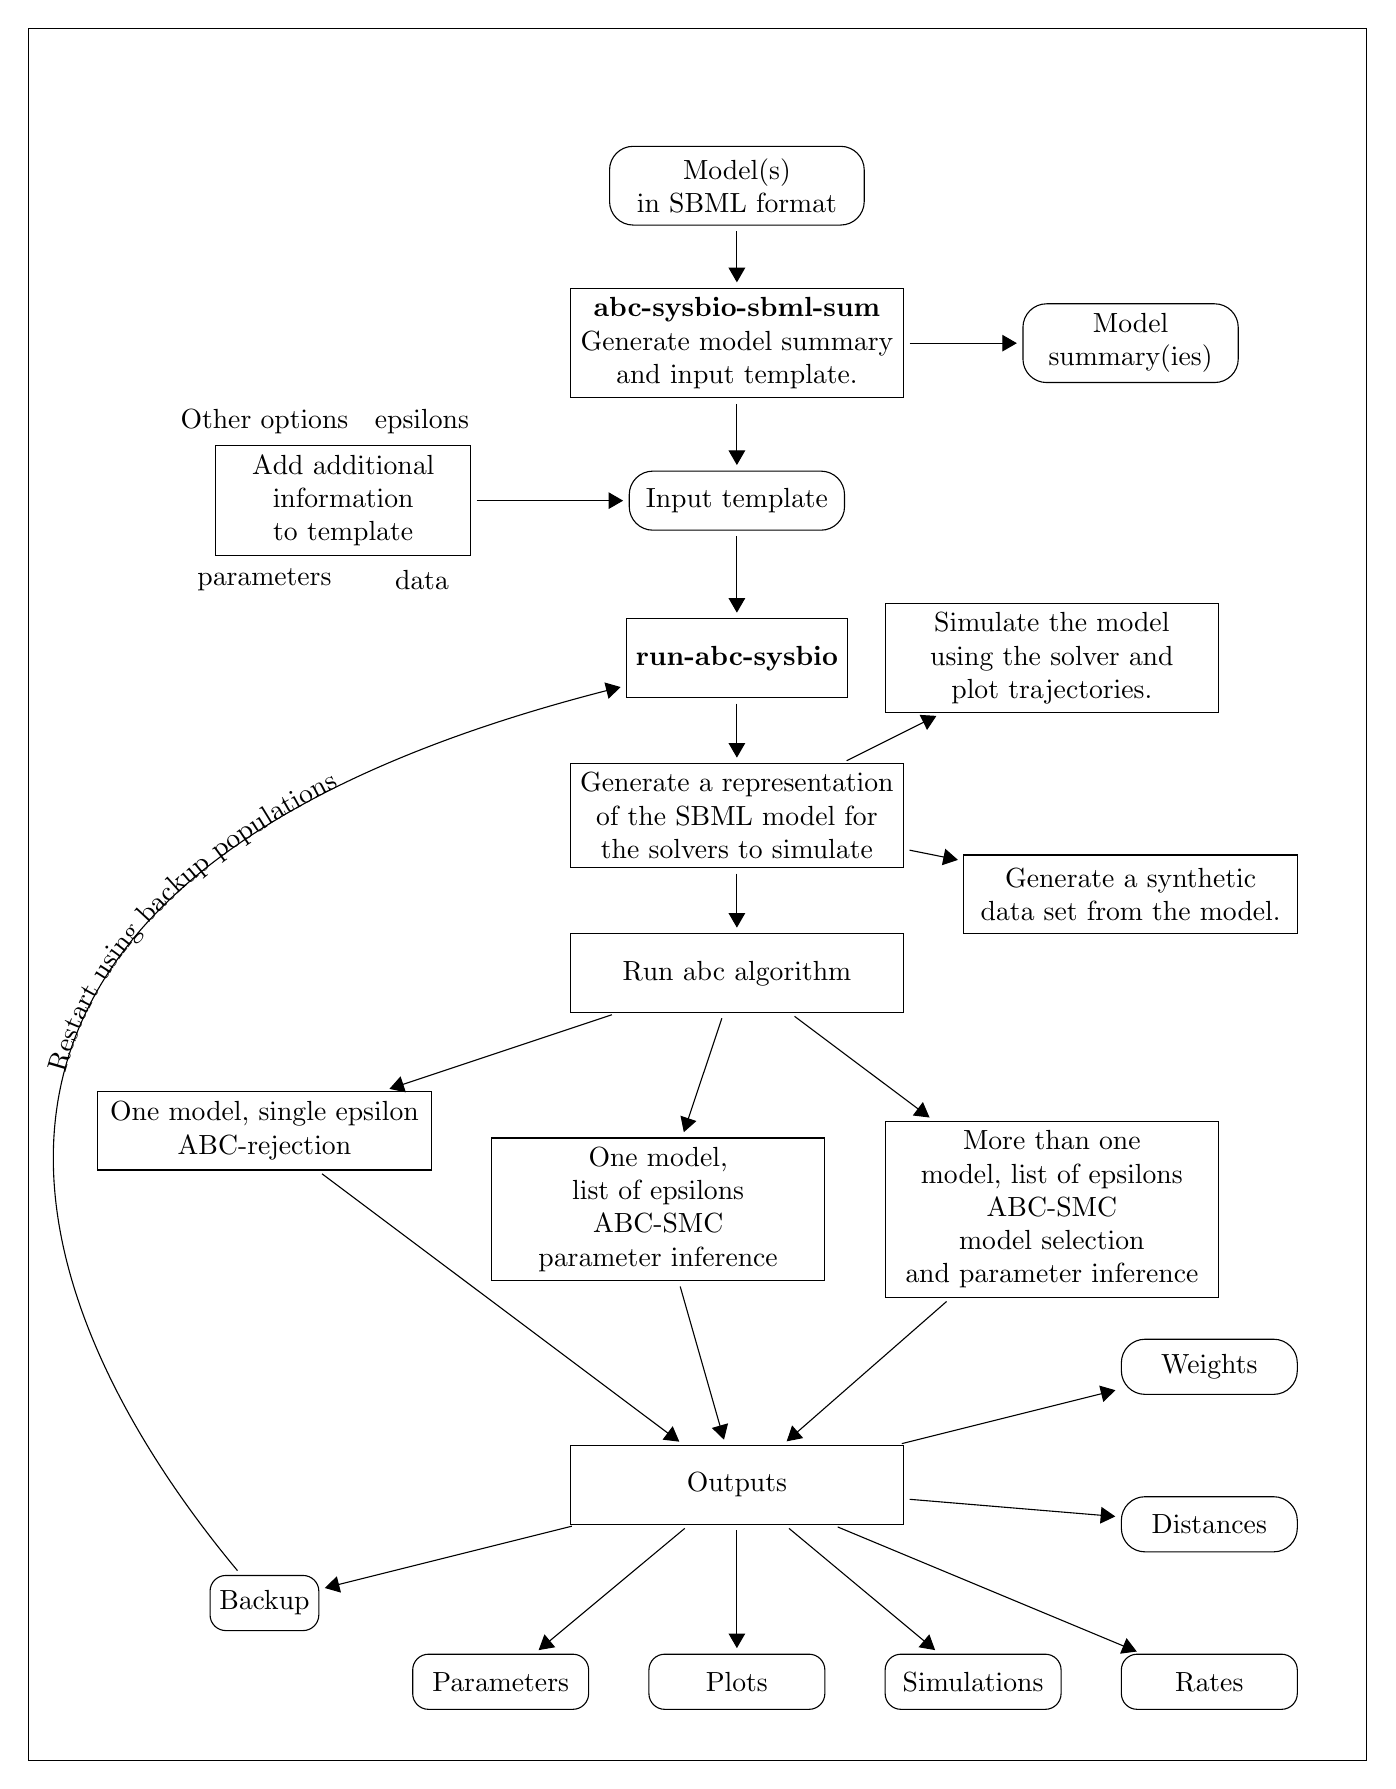
\begin{tikzpicture}

\draw[use as bounding box] (-3,0) rectangle (14,  22);
[line width=2pt]
[>=triangle 60]
%[show background rectangle]

Boxes
\draw (6,20) node [minimum size=1cm,rectangle, rounded corners = 3mm,draw,text width = 3cm, text centered] (Models)  {Model(s)\\in SBML format};
\draw (6,18) node [minimum size=1cm,rectangle,draw,text centered,text width=4cm] (generateTemplate) {{\bf abc-sysbio-sbml-sum}\\Generate model summary and input template.};
\draw (11,18) node [minimum size=1cm,rectangle, draw, rounded corners = 3mm, text centered,text width=2.5cm] (modelSummary) {Model\\summary(ies)};
\draw (6,16) node [minimum size=0.75cm,rectangle,draw, rounded corners = 3mm,text centered,text width=2.5cm] (inputTemplate) {Input template};
\draw (1, 16) node [minimum size=1cm,rectangle,draw,text centered,text width=3cm] (info) {Add additional information to template};
\draw (0, 15) node [text centered] (Parameters) {parameters};
\draw (2, 15) node [text centered] (Data) {data};
\draw (2, 17) node [text centered] (Epsilons) {epsilons};
\draw (0, 17) node [text centered] (otherOptions) {Other options};
\draw (6,14) node [minimum size=1cm,rectangle,draw,text centered] (abcScript) {{\bf run-abc-sysbio}};
\draw (6, 12) node [minimum size=1cm,rectangle, draw,text width = 4cm, text centered] (pythonModels)  {Generate a representation of the SBML model for the solvers to simulate};
\draw (10, 14) node [minimum size=1cm,rectangle, draw,text width = 4cm, text centered] (simulate) {Simulate the model using the solver and plot trajectories.};
\draw (11, 11) node [minimum size=1cm,rectangle, draw,text width = 4cm, text centered] (synthetic) {Generate a synthetic data set from the model.};
\draw (6, 10) node [minimum size=1cm,rectangle, draw,text width = 4cm, text centered] (run)  {Run abc algorithm};
\draw (0, 8) node [minimum size=1cm,rectangle, draw,text width = 4cm, text centered] (abcRejection)  {One model, single epsilon\\ABC-rejection};
\draw (5, 7) node [minimum size=1cm,rectangle, draw,text width = 4cm, text centered] (abcSMCParam)  {One model, list of epsilons\\ABC-SMC\\parameter inference};
\draw (10, 7) node [minimum size=1cm,rectangle, draw,text width = 4cm, text centered] (abcSMCModel)  {More than one model, list of epsilons\\ABC-SMC model selection\\and parameter inference};
\draw (6, 3.5) node [minimum size=1cm,rectangle, draw,text width = 4cm, text centered] (outputs) {Outputs};

Outputs
\draw (0, 2) node [minimum size = 7mm, rectangle, draw, text centered, rounded corners = 2mm] (backup) {Backup};
\draw (3, 1) node [minimum size=7mm,rectangle, draw,text width = 2cm, text centered, rounded corners = 2mm] (parameters) {Parameters};
\draw (6, 1) node [minimum size=7mm,rectangle, draw,text width = 2cm, text centered, rounded corners = 2mm] (plots) {Plots};
\draw (9, 1) node [minimum size=7mm,rectangle, draw,text width = 2cm, text centered, rounded corners = 2mm] (simulations) {Simulations};
\draw (12, 1) node [minimum size=7mm,rectangle, draw,text width = 2cm, text centered, rounded corners = 2mm] (rates) {Rates};
\draw (12, 3) node [minimum size = 7mm, rectangle, draw, text width = 2cm, text centered, rounded corners = 3mm] (distances) {Distances};
\draw (12, 5) node [minimum size = 7mm, rectangle, draw, text width = 2cm, text centered, rounded corners = 3mm] (weights) {Weights};

Lines
\draw [->,-triangle 60, shorten >= 2pt, shorten <=2pt] (Models)--(generateTemplate);
\draw [->,-triangle 60, shorten >=2pt, shorten <=2pt] (generateTemplate)--(modelSummary);
\draw [->,-triangle 60,shorten >=2pt, shorten <=2pt] (generateTemplate)--(inputTemplate);
\draw [->,-triangle 60,shorten >=2pt, shorten <=2pt] (info)--(inputTemplate);
\draw [->,-triangle 60,shorten >=2pt, shorten <=2pt] (inputTemplate)--(abcScript);
\draw [->,-triangle 60,shorten >=2pt, shorten <=2pt] (abcScript)--(pythonModels);
\draw [->,-triangle 60,shorten >=2pt, shorten <=2pt] (pythonModels)--(simulate);
\draw [->,-triangle 60,shorten >=2pt, shorten <=2pt] (pythonModels)--(synthetic);
\draw [->,-triangle 60,shorten >=2pt, shorten <=2pt] (pythonModels)--(run);
\draw [->,-triangle 60,shorten >=2pt, shorten <=2pt] (run)--(abcRejection);
\draw [->,-triangle 60,shorten >=2pt, shorten <=2pt] (run)--(abcSMCParam);
\draw [->,-triangle 60,shorten >=2pt, shorten <=2pt] (run)--(abcSMCModel);
\draw [->,-triangle 60,shorten >=2pt, shorten <=2pt] (abcRejection)--(outputs);
\draw [->,-triangle 60,shorten >=2pt, shorten <=2pt] (abcSMCParam)--(outputs);
\draw [->,-triangle 60,shorten >=2pt, shorten <=2pt] (abcSMCModel)--(outputs);
\draw [->,-triangle 60,shorten >=2pt, shorten <=2pt, postaction={decorate,decoration={text along path,text={Restart using backup populations}, pre length=7cm}}] (backup) .. controls (-2.5,5) and (-6, 11) .. (abcScript);

\draw [->,-triangle 60, shorten >= 2pt, shorten <=2pt] (outputs)--(backup);
\draw [->,-triangle 60, shorten >= 2pt, shorten <=2pt] (outputs)--(parameters);
\draw [->,-triangle 60, shorten >= 2pt, shorten <=2pt] (outputs)--(plots);
\draw [->,-triangle 60, shorten >= 2pt, shorten <=2pt] (outputs)--(simulations);
\draw [->,-triangle 60, shorten >= 2pt, shorten <=2pt] (outputs)--(rates);
\draw [->,-triangle 60, shorten >= 2pt, shorten <=2pt] (outputs)--(distances);
\draw [->,-triangle 60, shorten >= 2pt, shorten <=2pt] (outputs)--(weights);
\end{tikzpicture}

\end{center}
\end{document}